\section{Vorläufige Realisierung}
\label{sec:realisierung}

[Wagner96] zeigt mehrere Diagramme. Eine Untersuchung der realen Spurwechselvorgänge ergab, dass eine Umkehr der Benutzungshäufigkeit der rechten und linken Spuren bei einem Verkehrsfluss $q_{12}$ von etwa 1200 (Fahrzeugen) pro Stunde auf beiden Spuren.

Die Simulation ergab, dass der Punkt, an dem beide Spuren gleichermaßen benutzt werden, deutlich unter dem Punkt liegt, an dem der maximale Verkehrsfluss erreicht wird, siehe \cref{figure:verkehrsfluss-spurnutzung}.

\begin{figure}[h]
 \centering
 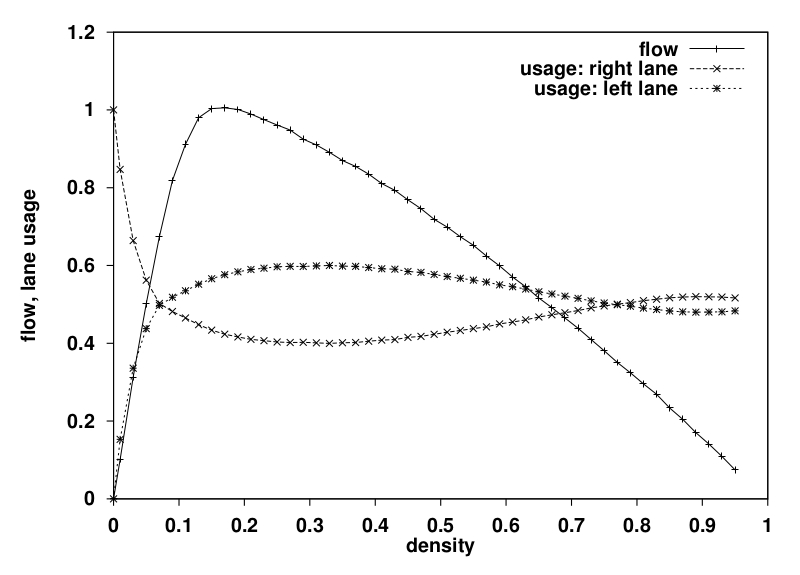
\includegraphics[width=0.75\textwidth]{verkehrsfluss-spurnutzung}
 \caption[Verkehrsfluss und Spurnutzung als Funktion der Verkehrsdichte]{Verkehrsfluss und Spurnutzung als Funktion der Verkehrsdichte, aus [Wagner96]}
 \label{figure:verkehrsfluss-spurnutzung}
\end{figure}

Ein weiteres Resultat der Simulation ist eine mehrfache Umkehr der Nutzung der Fahrspuren abhängig von der Verkehrsdichte, wenn andere Parameter konstant gehalten werden, siehe \cref{figure:verkehrsfluss}.

\begin{figure}[h]
 \centering
 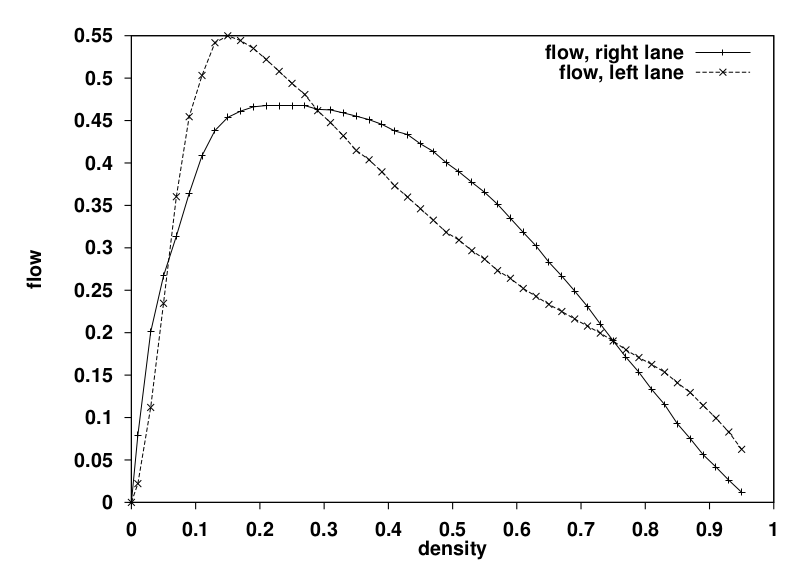
\includegraphics[width=0.75\textwidth]{verkehrsfluss}
 \caption[Verkehrsfluss als Funktion der durchschnittlichen Verkehrsdichte]{Verkehrsfluss auf den Fahrspuren als Funktion der durchschnittlichen Verkehrsdichte, aus [Wagner96]}
 \label{figure:verkehrsfluss}
\end{figure}

Die Festlegung einer Wahrscheinlichkeit für das Zurückwechseln von der linken auf die rechte Fahrspur führte zu einer unterschiedlichen Spurwechselfrequenz, siehe \cref{figure:spurwechselfrequenz}.

\begin{figure}[h]
 \centering
 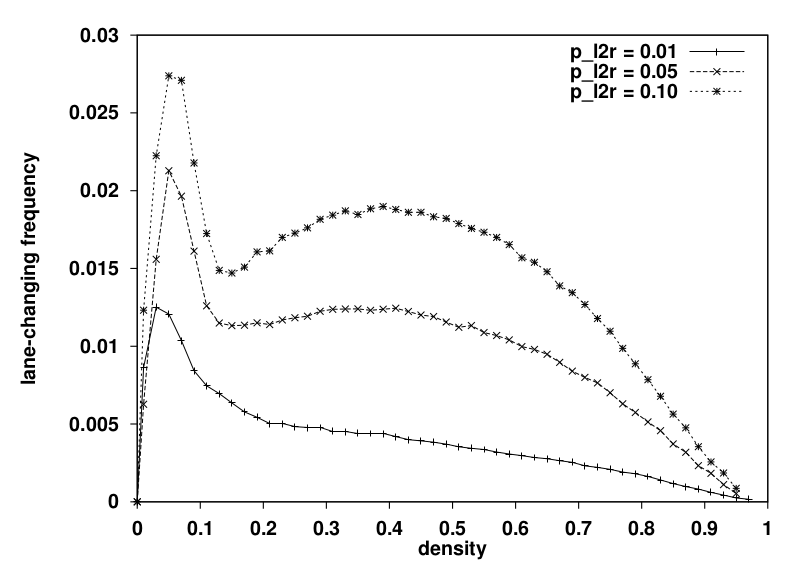
\includegraphics[width=0.75\textwidth]{spurwechselfrequenz}
 \caption[Spurwechselfrequenz als Funktion der Verkehrsdichte]{Spurwechselfrequenz als Funktion der Verkehrsdichte für verschiedene Spurwechselwahrscheinlichkeiten, aus [Wagner96]}
 \label{figure:spurwechselfrequenz}
\end{figure}

Die in [Tran17] vorgeschlagene Struktur ist zu implementieren und in entsprechend vergleichbarer Umgebung simulatorisch zu testen. Dabei sind die folgenden Größen zu erheben und in entsprechend statistisch auszuwerten: Verkehrsdichte, Verkehrsfluss, Spurwechselfrequenz und Spurnutzung links/rechts.